% 1986 年广东卷理工农医类第二卷第二题：直线与两平面关系示意图。
% 按固定源 PDF 第 5 页重绘；第二幅原图中 E 的交叠位置不作为空间交点解释。
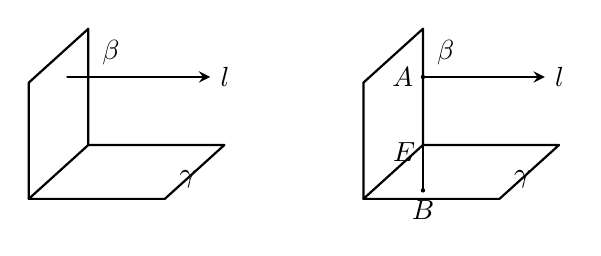
\begin{tikzpicture}[>=stealth, line cap=round, line join=round]
  % 图一：两个相交平面及平行于 gamma、垂直于 beta 的直线 l。
  \begin{scope}[xshift=0cm, scale=0.72]
    \coordinate (O) at (0,0);
    \coordinate (X) at (2.4,0);
    \coordinate (Y) at (1.05,0.95);
    \coordinate (XY) at (3.45,0.95);
    \coordinate (T) at (1.05,3.0);
    \coordinate (L0) at (0.68,2.15);
    \coordinate (L1) at (3.2,2.15);
    \draw[thick] (O)--(X)--(XY)--(Y)--cycle;
    \draw[thick] (O)--(0,2.05)--(T)--(Y);
    \draw[thick] (Y)--(T);
    \draw[thick,->] (L0)--(L1) node[right] {$l$};
    \node at (1.45,2.58) {$\beta$};
    \node at (2.8,0.35) {$\gamma$};
  \end{scope}

  % 图二：加入 A、B 及原图标记 E；不将示意图中的重叠点解释为
  % AB 与 m 的几何交点（A 不在 gamma 内，B 已在 gamma 内）。
  \begin{scope}[xshift=4.25cm, scale=0.72]
    \coordinate (O) at (0,0);
    \coordinate (X) at (2.4,0);
    \coordinate (Y) at (1.05,0.95);
    \coordinate (XY) at (3.45,0.95);
    \coordinate (T) at (1.05,3.0);
    \coordinate (A) at (1.05,2.15);
    \coordinate (B) at (1.05,0.15);
    \coordinate (L1) at (3.2,2.15);
    \draw[thick] (O)--(X)--(XY)--(Y)--cycle;
    \draw[thick] (O)--(0,2.05)--(T)--(Y);
    \draw[thick] (Y)--(T);
    \draw[thick,->] (A)--(L1) node[right] {$l$};
    \draw[thick] (A)--(B);
    \fill (A) circle (1.1pt) node[left] {$A$};
    \fill (B) circle (1.1pt) node[below] {$B$};
    \node at (1.45,2.58) {$\beta$};
    \node at (2.8,0.35) {$\gamma$};
    \node at (0.72,0.83) {$E$};
  \end{scope}
\end{tikzpicture}
